\chapter{指针与地址}

\section{指针的本质}

指针是 C语言最核心也最强大的特性。指针变量存储的是另一个变量的\textbf{内存地址}，而非数据本身。

\begin{lstlisting}[caption={指针基础示例}]
int a = 10;
int *p = &a;    // p 存储的是 a 的内存地址
printf("%p\n", (void*)p);   // 打印地址
printf("%d\n", *p);         // 解引用：通过地址获取值，输出 10
\end{lstlisting}

\begin{itemize}
    \item \texttt{\&}（取地址符）：获取变量的内存地址。
    \item \texttt{*}（解引用符/间接寻址符）：通过指针访问其所指向地址中存储的值。
    \item 指针本身也是一个变量，它有自己的内存地址和所占空间（32位系统为 4 字节，64位系统为 8 字节）。
\end{itemize}

\begin{figure}[H]
\centering
\begin{tikzpicture}[
    box/.style={draw, minimum width=1.8cm, minimum height=0.9cm, align=center, font=\ttfamily},
    arrow/.style={->, >=latex, thick},
    lbl/.style={font=\small}
]
    % 变量 a
    \node[box] (a) at (0,0) {a = 10};
    \node[lbl, above] at (a.north) {地址: 0x1000};
    % 指针 p
    \node[box, fill=yellow!20] (p) at (4,0) {p};
    \node[lbl, above] at (p.north) {地址: 0x2000};
    \node[lbl, below] at (p.south) {值: 0x1000};
    % 指针指向
    \draw[arrow, red] (p.west) -- node[lbl, above] {指向} (a.east);
\end{tikzpicture}
\caption{指针变量 p 指向变量 a 的内存关系图}
\label{fig:pointer_basic}
\end{figure}

\section{指针与数组的关系}

在 C语言中，数组名本质上就是指向数组首元素的常量指针。

\begin{lstlisting}[caption={指针与数组}]
int arr[5] = {1, 2, 3, 4, 5};
int *p = arr;       // 等价于 int *p = &arr[0];
printf("%d", *(p + 2)); // 输出 3，等价于 arr[2]
\end{lstlisting}

\textbf{指针算术运算}：指针加减整数时，实际移动的字节数 = 整数值 $\times$ \texttt{sizeof(指针指向的类型)}。

\begin{figure}[H]
\centering
\begin{tikzpicture}[
    cell/.style={draw, minimum width=1.3cm, minimum height=0.75cm, font=\ttfamily},
    arrow/.style={->, >=latex, thick},
    lbl/.style={font=\small}
]
    \matrix (arr) [matrix of nodes, nodes={cell}, column sep=-\pgflinewidth] {
        1 & 2 & 3 & 4 & 5 \\
    };
    \node[lbl] at ($(arr-1-1.south)+(0,-0.35)$) {arr[0]};
    \node[lbl] at ($(arr-1-2.south)+(0,-0.35)$) {arr[1]};
    \node[lbl] at ($(arr-1-3.south)+(0,-0.35)$) {arr[2]};
    \node[lbl] at ($(arr-1-4.south)+(0,-0.35)$) {arr[3]};
    \node[lbl] at ($(arr-1-5.south)+(0,-0.35)$) {arr[4]};
    % p 指向 arr[0]
    \node[lbl, anchor=south] (ptr) at ($(arr-1-1.north)+(0,0.5)$) {p (指向 arr[0])};
    \draw[arrow] (ptr.south) -- (arr-1-1.north);
    % p+2 指向 arr[2]
    \node[lbl, anchor=south] (ptr2) at ($(arr-1-3.north)+(0,1.0)$) {p+2 (指向 arr[2])};
    \draw[arrow] (ptr2.south) -- (arr-1-3.north);
\end{tikzpicture}
\caption{指针算术运算与数组内存布局}
\label{fig:pointer_array}
\end{figure}

\section{指针与字符串}

C语言中的字符串是以 \texttt{\textbackslash 0} 结尾的字符数组。字符串字面量在内存中以只读方式存储，返回指向首字符的指针。

\begin{lstlisting}[caption={指针与字符串}]
char *str = "Hello";    // str 指向字符串字面量的首地址
printf("%c\n", *str);   // 输出 'H'
printf("%c\n", *(str+1)); // 输出 'e'

// 注意：不可修改字符串字面量
// str[0] = 'h';        // 未定义行为，可能导致段错误
\end{lstlisting}

\section{多级指针}

指针可以指向另一个指针，形成多级间接寻址。二级指针常用于修改指针本身的值（如动态分配二维数组、修改函数外部的指针变量）。

\begin{lstlisting}[caption={二级指针示例}]
int a = 10;
int *p = &a;
int **pp = &p;

printf("%d\n", *p);     // 输出 10，一次解引用
printf("%d\n", **pp);   // 输出 10，两次解引用

**pp = 20;              // 通过二级指针修改 a 的值
printf("%d\n", a);      // 输出 20
\end{lstlisting}

\begin{figure}[H]
\centering
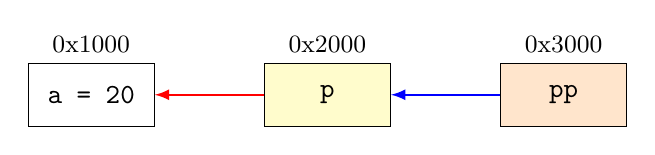
\begin{tikzpicture}[
    box/.style={draw, minimum width=1.6cm, minimum height=0.8cm, align=center, font=\ttfamily},
    arrow/.style={->, >=latex, thick},
    lbl/.style={font=\small}
]
    \node[box] (a) at (0,0) {a = 20};
    \node[box, fill=yellow!20] (p) at (3,0) {p};
    \node[box, fill=orange!20] (pp) at (6,0) {pp};
    \draw[arrow, red] (p.west) -- (a.east);
    \draw[arrow, blue] (pp.west) -- (p.east);
    \node[lbl, above] at (a.north) {0x1000};
    \node[lbl, above] at (p.north) {0x2000};
    \node[lbl, above] at (pp.north) {0x3000};
\end{tikzpicture}
\caption{二级指针链式指向关系}
\label{fig:double_pointer}
\end{figure}

\section{动态内存管理}

C语言通过标准库 \texttt{<stdlib.h>} 提供在堆（Heap）上动态分配内存的能力。

\begin{itemize}
    \item \textbf{\texttt{malloc(size\_t size)}}：在堆上分配指定字节数的内存，返回 \texttt{void*}，内容未初始化（垃圾值）。
    \item \textbf{\texttt{calloc(size\_t n, size\_t size)}}：分配 $n$ 个大小为 \texttt{size} 的连续内存块，并自动初始化为 0。
    \item \textbf{\texttt{realloc(void* ptr, size\_t size)}}：重新调整已分配内存的大小。若新大小更大，原有数据保留，新增部分未初始化。
    \item \textbf{\texttt{free(void* ptr)}}：释放已分配的内存，防止内存泄漏。
\end{itemize}

\begin{lstlisting}[caption={动态内存管理示例}]
#include <stdlib.h>

int *arr = (int*)malloc(10 * sizeof(int));
if (arr == NULL) {
    // 内存分配失败处理
    return -1;
}

// 使用 arr...
arr[0] = 42;

// 使用完毕后必须释放
free(arr);
arr = NULL; // 避免悬垂指针（Dangling Pointer）
\end{lstlisting}

\textbf{关键注意事项}：

\begin{itemize}
    \item 每次 \texttt{malloc} 必须配对一次 \texttt{free}，否则造成内存泄漏。
    \item \texttt{free} 之后的指针应立即置为 \texttt{NULL}，避免悬垂指针被误用。
    \item 不可对同一块内存 \texttt{free} 两次（Double Free），会导致未定义行为。
\end{itemize}

\section{函数指针与回调}

函数指针允许将函数作为参数传递，实现回调机制和多态行为。

\begin{lstlisting}[caption={函数指针示例}]
int add(int a, int b) { return a + b; }
int sub(int a, int b) { return a - b; }

// 声明函数指针
int (*func_ptr)(int, int);

func_ptr = add;
printf("%d\n", func_ptr(3, 4)); // 输出 7

func_ptr = sub;
printf("%d\n", func_ptr(3, 4)); // 输出 -1
\end{lstlisting}

\begin{lstlisting}[caption={回调函数示例}]
// 通用排序比较函数原型
typedef int (*CompareFunc)(const void*, const void*);

void mySort(int arr[], int n, CompareFunc cmp) {
    // 排序过程中调用 cmp 比较元素
    for (int i = 0; i < n - 1; i++) {
        for (int j = 0; j < n - i - 1; j++) {
            if (cmp(&arr[j], &arr[j+1]) > 0) {
                int tmp = arr[j];
                arr[j] = arr[j+1];
                arr[j+1] = tmp;
            }
        }
    }
}
\end{lstlisting}

\section{\texttt{const} 与指针的组合}

\texttt{const} 修饰指针时有三种经典组合方式，含义各不相同：

\begin{lstlisting}[caption={const 与指针的三种组合}]
int a = 10, b = 20;

// 1. 指针常量：指针本身不可变，但指向的值可变
int *const p1 = &a;
*p1 = 30;     // OK
// p1 = &b;   // Error: p1 是常量

// 2. 常量指针：指向的值不可变，但指针本身可变
const int *p2 = &a;
// *p2 = 30;  // Error: *p2 是常量
p2 = &b;      // OK

// 3. 指向常量的常量指针：两者均不可变
const int *const p3 = &a;
// *p3 = 30;  // Error
// p3 = &b;   // Error
\end{lstlisting}

\textbf{记忆口诀}：\texttt{const} 在 \texttt{*} 左侧 $\to$ 值不可变；\texttt{const} 在 \texttt{*} 右侧 $\to$ 指针不可变。

\section{复杂指针声明解析}

在 C 语言中，指针与数组、函数的组合会产生复杂的声明。理解它们的关键是**从变量名开始，按照优先级向外结合**。

\subsection{指针数组 vs 数组指针}

\begin{figure}[H]
\centering
\begin{minipage}{0.95\textwidth}
\begin{lstlisting}[caption={指针数组与数组指针}]
int *p1[10];   // 指针数组：数组，包含 10 个 int* 指针
int (*p2)[10]; // 数组指针：指针，指向一个包含 10 个 int 的数组

// 解析技巧：
// [] 优先级高于 *，所以 p1 先和 [] 结合，是数组。
// () 强制优先级，所以 p2 先和 * 结合，是指针。
\end{lstlisting}
\end{minipage}
\end{figure}

\subsection{函数指针数组}

\begin{figure}[H]
\centering
\begin{minipage}{0.95\textwidth}
\begin{lstlisting}[caption={函数指针数组示例}]
int add(int a, int b) { return a + b; }
int sub(int a, int b) { return a - b; }

// 声明一个包含 2 个函数指针的数组
int (*ops[2])(int, int) = {add, sub};

printf("%d\n", ops[0](3, 4)); // 输出 7
printf("%d\n", ops[1](3, 4)); // 输出 -1
\end{lstlisting}
\end{minipage}
\end{figure}

\section{实战：单链表的 C 语言实现}

作为指针和结构体的综合练习，以下实现了一个带头结点的单链表，包含插入、删除和遍历操作。这是衔接《数据结构》课程的经典案例。

\begin{figure}[H]
\centering
\begin{minipage}{0.95\textwidth}
\begin{lstlisting}[caption={单链表完整实现}]
#include <stdio.h>
#include <stdlib.h>

// 节点定义
typedef struct Node {
    int data;
    struct Node *next;
} Node;

// 初始化带头结点的链表
Node* initList() {
    Node *head = (Node*)malloc(sizeof(Node));
    head->next = NULL;
    return head;
}

// 头插法
void insertHead(Node *head, int val) {
    Node *newNode = (Node*)malloc(sizeof(Node));
    newNode->data = val;
    newNode->next = head->next;
    head->next = newNode;
}

// 删除第一个值为 val 的节点
void deleteVal(Node *head, int val) {
    Node *prev = head;
    Node *curr = head->next;
    while (curr) {
        if (curr->data == val) {
            prev->next = curr->next;
            free(curr);
            return;
        }
        prev = curr;
        curr = curr->next;
    }
}

// 遍历打印
void printList(Node *head) {
    Node *curr = head->next;
    while (curr) {
        printf("%d -> ", curr->data);
        curr = curr->next;
    }
    printf("NULL\n");
}

// 释放整个链表
void freeList(Node *head) {
    Node *curr = head;
    while (curr) {
        Node *tmp = curr;
        curr = curr->next;
        free(tmp);
    }
}
\end{lstlisting}
\end{minipage}
\end{figure}
